%% This is an example first chapter.  You should put chapter/appendix that you
%% write into a separate file, and add a line \include{yourfilename} to
%% main.tex, where `yourfilename.tex' is the name of the chapter/appendix file.
%% You can process specific files by typing their names in at the 
%% \files=
%% prompt when you run the file main.tex through LaTeX.
\chapter{Conclusion for Our Analysis}

\chapter{Extension:Low-threshold detector development}

\begin{comment}
\section{\label{sec:level1}Introduction:\protect\\
Why GeIA? and The issue}

For the exploration of the lower-mass region for WIMPs, the first immediate idea is "Since the signal of WIMP is so small, why don't we just amplify it?" Some people commenced their contemplation on the technical works.\\

In 2000, two smart Russian guys came up with the brilliant idea about applying the high voltage on the Ge detector, and the signal will be amplified by the avalanche region emerging in the crystal under the high voltage. Now, there are a bunch of experiments trying to extend the idea and to see whether it can be worked out with the more state-of-the-art technique.\\ 

Although the internal amplification seems a good idea, the noise of the crystal could be unexpectedly amplified as well. Dealing with the issue of the high noise originating from the leakage current is another topic for this experiment. In this document, we will also confirm the issue of the noise in the crystal.\\

In our collaborations, we have two teams working on the idea under two conventional temperatures, which are 4K(USD) and 77K(THU). I would like to explore that under these two temperatures, what will happen to the crystal from the perspective of "the signal" and also "the noise" under the high voltage.


%%%%%%%%%%%%%%%%%%%%%%%%%%%%%%%%%%%%%%%%%%%%%%%%%%%%%%%%

\section{\label{sec:level2}Basic p-n junction}
Given the semiconductor containing the different types of impurity, we can get two groups, including the n(electron-dominant) and p(hole-dominant) types. For any crystal containing both types of semiconductors, the properties of the p-n junction will occur by and large. I would like to briefly discuss the phenomenon for it.\\

On the p-n junction, the electron-hole diffusion, as well as the attraction, will start emerging in the crystal. After the "dynamic" get balance, the neutral region called "the depletion region" that the stable electric field flows in will show up. In the reverse-bias case, the higher the voltage, the bigger the region it will be. In the end, we need to increase the voltage to the one which can deplete all the crystal, meaning that all electrons and holes in the crystal get balance. Then, we can start our usage of the crystal.\\

If you want to know more details about the fundamental physics in semiconductor, I recommend the book\cite{10.5555/1594006}, chapter7 and chapter8, or wiki page.

%%%%%%%%%%%%%%%%%%%%%%%%%%%%%%%%%%%%%%%%%%%%%%%%%%%%%%%%

\section{\label{sec:level3}signal amplification}

\subsection{From the perspective of "an electron":}
At the start, let us imagine "an electron", which is ionized by a WIMP,  flowing in the crystal. There are many important parameters that we should acquire from it for opening our studies. I will depict them in the following paragraph.

\begin{enumerate}
	\item Electrical Mobility($\mu$): Related to the conductivity of the electron in the crystal. In the paper\cite{7}, basically, all of the important information is included. From the formula2 of paper\cite{7}, which is used to summarize the mobility, we can see that the smaller the individual mobility, the higher the importance that is. From our research, actually, the acoustic phonon scattering is the dominant term for 77K, and the neutral impurity scattering, which is not affected by the temperature normally, is the dominant term for 4K. You can compare between Fig.2 and Fig.3 in the paper\cite{7}.
	\item Effective mass(m*): Under the different temperatures, the conductivity effective masses are various. Fig.5. of the paper\cite{6} describes the effective mass with respect to the temperature. Since there is no such study for Ge, we just take Si as our standard in this case to give us a sense on the tendency of it.
	\item Relaxation Time($\tau$): The period of time that the electron can run without bumping into another atom. You can also find out the formula in the paper\cite{7}.
	
	\begin{equation}
    \tau = \frac{\mu \times m*}{e}
    \end{equation}
	e is the coulomb constant\\
	
	After acknowledging the relaxation time, the next thing we need to figure out is the mean free path($\L$). which means how far the electron can go without colliding with another atom in the crystal. The formula is as follows:
\begin{equation}
\label{MFP}
L = \tau \times V_{d}
\end{equation}
$V_{d}$ means the velocity of the electron. 
	\item electron velocity($V_{d}$): The relation between the velocity of the electron and the voltage applied to the crystal is demonstrated in Fig.1 of the paper\cite{5}. 
\end{enumerate}

After all of the parameters are well-recognized in this section, we will use some of them in the next section and start our journey on the amplification. 




\subsection{Ionization rate}
The definition of ionization rate: How many electrons/holes can be ionized within 1cm?\\

After depleting the crystal, next we would like to ask the relation between the ionization rate and the E(V/cm). Based on the formula(20a) in \cite{2}, which can determine the ionization rate by figuring out mean free path(L), electric field(E(x)) and ionization energy(U) of the material, we can get FIG.\ref{fig1}. There are three important pieces of information given by this:\\

\begin{figure}[h]
  \centering
  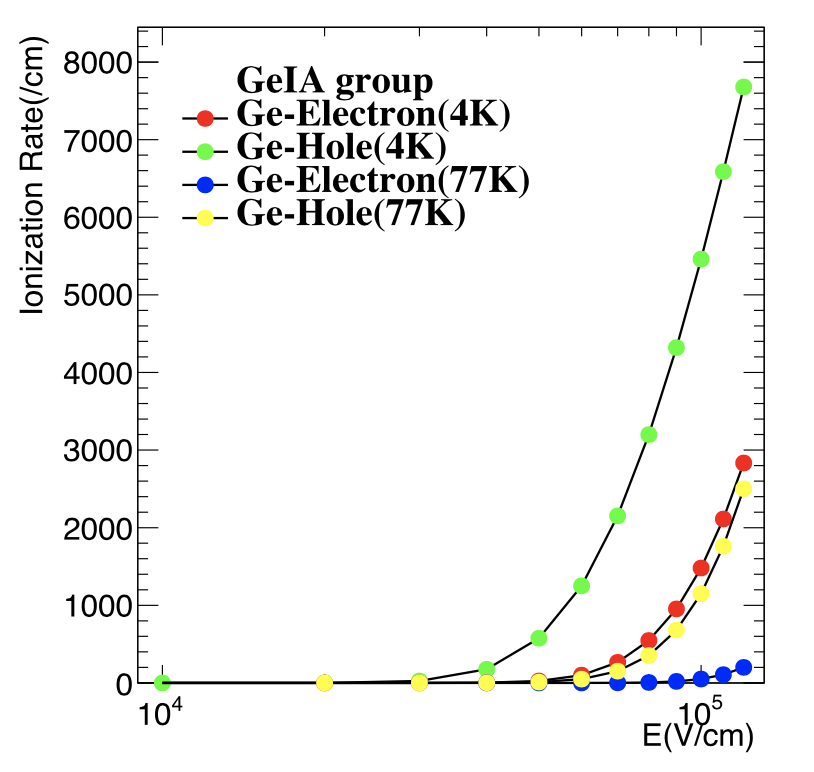
\includegraphics[width=0.35\textwidth]{SHEME/Ionization_rate.png}
  \caption{The ionization rates for both electron and hole under both 4K and 77K.}
  \label{fig1}
\end{figure}

\begin{enumerate}
	\item Critical E=$10^{4}$ V/cm
	\item The significant difference between e/h cases is the effective mass under such high electric field at the same T.
	\item Hole can give us more signal under the lower T.
\end{enumerate}

\subsection{Pioneer: Russian investigation[2000]}
In light of the paper\cite{1}, the conceptual design on the coaxial detector HPGe with the impurity of the crystal is provided. The key point is as the following sentence.\\ 

According to FIG.\ref{fig1}, when the electric field is higher than $10^{4}$(V/cm), the electron will be increased as the function of the electric field. Because of that, there are two regions that can be marked in FIG.2, given by Fig. 1 of the paper\cite{1}:

\begin{figure}[h]
  \centering
  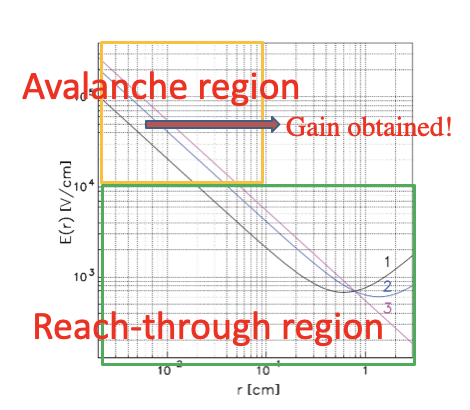
\includegraphics[width=0.35\textwidth]{SHEME/Avalanche_Reach_Through.png}
  \caption{The electric field as a function of the distance from the strip with the different impurities. The number above the lines mean the different impurities: (1)$10^{10} cm^{-3}$, (2)4 $\times 10^{9} cm^{-3}$ and (3) 0 $cm^{-3}$}
  \label{fig2}
\end{figure}

\begin{enumerate}
	\item Avalanche region: When the electric field is above $10^{4}$(V/cm), the avalanche effect will emerge, and the signal will be amplified. 
	\item Reach-through region: Below that, since the electron/hole will just go through normally without any effect on them.
\end{enumerate}

These studies give us a clue that we can devise a detector that can produce the amplification for the signal with the electric field above a certain level.
%%%%%%%%%%%%%%%%%%%%%%%%%%%%%%%%%%%%%%%%%%%%%%%%%%%%%%%%

\section{\label{sec:level3}noise in the crystal}
Unfortunately, the noise in the crystal is inevitable. The genres of the noise in the crystal should be characterized as the criteria of acquiring the feasibility of measuring dark matter theoretically. 
There are three kinds of noise in the crystal, encompassing the bulk leakage current, the contact leakage current, and the surface leakage current. In the following paragraph, I will depict them individually.\\

\subsection{Bulk leakage current}
Because of the thermal fluctuation, the electrons from the bulk(purity, such as Ge) material will be ionized possibly. Fortunately, the level of this noise can be ignored below 77K. The associated information is well-written in the formula(6) of paper\cite{doi:10.1063/1.4953147}. We can use the formula as follows to estimate the current.
\begin{equation}
I = A e^{\frac{-E_{Ge Band}}{2k_{B}T}}*q
\end{equation}
A=intrinsic concentration, $E_{Ge Band}$=Ge bandgap, q=coulomb constant, T= temperature(K)
\subsection{Contact leakage current}
Because of 
\begin{enumerate}
	\item The barrier between the semi-metal connection
	\item The thermal fluctuation
\end{enumerate}
There is a possibility that the electron in the conductive band of the semiconductor could jump into the metal, leading to the dark current which is unwanted. Fig.8 of the paper\cite{LOOKER2015138} and Fig. 10 of the paper\cite{Wei_2018} perform the leakage current at the different temperatures. The current at a certain temperature can be predicted by these two figures. \\

The fundamental physics is "Schottky effect", which is a kind of the thermal emission. We can express the simplified formula with the "Richardson's law" as follows: 
\begin{equation}
I \propto T^{2} e^{\frac{W}{k_{B}T}}
\end{equation}
$E_{Ge Band}$=Ge band gap q=coulomb constant 
T= temperature(K), W= work function of the material, A=Measured constant\\

You can find out the detail in the book\cite{10.5555/1203347}. This leakage current will be the dominant one under 77K.\\

Basically, it is a Metal-Semiconductor junction problem, which is a very big topic authentically and you can see the chapter 10, 11 of book\cite{10.5555/1203347}(Strongly recommended!) and chapter 6 and 7 of book\cite{MILNES1972171} for more detail.\\

\subsection{Surface leakage current}
It depends on the quality of the crystal. Although lowering the temperature will help decrease the noise, the mechanism of this current is not clear for now. We can only rely on the measurement.\\ 

There is a paper on measuring the surface leakage current for the semiconductor. Please look at Fig.2 of the paper\cite{5871995}. You can extend the points in the figure to predict the surface leakage current. Although it is not for Ge, it can give us a hint on the scale of the surface leakage current for semiconductors. This leakage current will be the dominant one under 4K.


\section{Conclusion and dilemma}

\begin{enumerate}
	\item If we can suppress the surface leakage current, we can get the lower threshold detector. But unfortunately, now there is no good way to decrease it. 
	\item Under the high temperature, such as 77K, the crystal could easily break down because of the high leakage current, now we would like to start with the experiment under 4K to produce a first version stable amplification. 
\end{enumerate}


\bibliographystyle{apsrev4-2} % Tell bibtex which bibliography style to use
\bibliography{GeIANotes_Used}
\end{comment}



